% arara: xelatex
%!TEX TS-program = xelatex
\documentclass[a4paper]{adcv}
\usepackage{comment}

\newcommand*{\hib}{}
\newcommand*{\uib}{}
\newcommand*{\uniaq}{}

\addbibresource{musty_cv.bib}

\title{musty_cv}

\adcvname{Michael Musty}{}
\adcvtitle{Ph.D. Candidate, Mathematics, Dartmouth College}
\adcvaddress{55 Church Street}{03779}{Piermont}{New Hampshire USA}
%\adcvwebsite{https://math.dartmouth.edu/~mjmusty}{math.dartmouth.edu/~mjmusty}
%\adcvwebsite{https://michaelmusty.github.io}{michaelmusty.github.io}
\adcvwebsite{https://github.com/michaelmusty}{https://github.com/michaelmusty}
\adcvemail{michaelmusty}{gmail}{com}
\adcvphone{(+1) 603 728 7903}
\adcvdate{December 2018}
\adcvlinkedin{https://www.linkedin.com/in/mjmusty/}{https://www.linkedin.com/in/mjmusty}

\begin{document}

\section{Education}{
  \begin{adcvtabletwo}
    \adcvrowtwo{\textbf{Ph.D. Mathematics}, Dartmouth College, Hanover, New Hampshire, USA}{expected 2019}
    \adcvrowskip
    \adcvrowtwo{\textbf{M.Sc. Mathematics}, University of Vermont, Burlington, Vermont, USA}{2014}
    \adcvrowskip
    \adcvrowtwo{\textbf{B.A. Mathematics/Scientific Computing}, Boston College, Chestnut Hill, Massachusetts, USA}{2008}
  \end{adcvtabletwo}
}

\section{Research Experience}{
  \begin{adcvtabletwo}
    \adcvrowtwo{\textbf{2-Group Belyi Maps}, Ph.D. Thesis}{expected 2019}
      \vspace{-10pt}
      \begin{itemize}
        \item
          Developed and implemented an algorithm to compute
          a database of 2-group Belyi maps up to degree 256
        \item
          Analyzed this data to steer conjectures about these objects
        \item
          Used this analysis to search for special number fields
          ramified only at 2
        \item
          Repository: \url{https://github.com/michaelmusty/solvabledessins}
        \item
          Visualization: \url{https://dessin-explorer.org}
      \end{itemize}
    \adcvrowskip
    \adcvrowtwo{\textbf{Computing Canonical Rings of Hilbert Modular Forms}, Programmer}{2018}
      \vspace{-10pt}
      \begin{itemize}
        \item
          Implemented the data structure to store
          and compute with Fourier expansions of Hilbert modular forms
        \item
          Worked as part of a 10+ person team
        \item
          Organized the (git) workflow of the team
        \item
          Repository: \url{https://github.com/edgarcosta/hilbertmodularforms}
      \end{itemize}
    \adcvrowskip
    \adcvrowtwo{\textbf{A Database of Belyi Maps}, Co-author}{2018}
      \vspace{-10pt}
      \begin{itemize}
        \item
          Implemented the database backend using Magma
        \item
          Computed thousands of Belyi maps up to degree 9
        \item
          Worked in a team of 4 people to migrate this data over
          to the LMFDB (\url{www.lmfdb.org})
        \item
          Wrote Magma and Python scripts to convert this Magma database
          to MongoDB as part of the migration
        \item
          Awarded Selfridge Prize at ANTS-XIII:
          \url{http://www.math.grinnell.edu/~paulhusj/ants2018/index.html}
        \item
          Repository: \url{https://github.com/michaelmusty/BelyiDB}
        \item
          LMFDB: \url{http://beta.lmfdb.org/Belyi}
        \item
          Peer-Reviewed Article: \cite{ants}
      \end{itemize}
    \adcvrowskip
    \adcvrowtwo{\textbf{Understanding the cost of dermatologic care: A survey study of dermatology providers,
    residents, and patients}, Co-author}{2017}
      \vspace{-10pt}
      \begin{itemize}
        \item
          Carried out the statistical analysis for survey data of this study
          using R
        \item
          Generated Likert scale visualizations to analyze the study data
          using R
        \item
          Peer-Reviewed Article: \cite{aaron}
      \end{itemize}
    \adcvrowskip
    \adcvrowtwo{\textbf{Numerical calculation of three-point branched covers of the projective line},
    Co-author}{2014}
      \vspace{-10pt}
      \begin{itemize}
        \item
          Implemented a general numerical method to compute
          Belyi maps using power series expansions of modular forms
        \item
          Implemented code to visualize dessins d'enfants
          (equivalent objects to Belyi maps) conformally embedded in
          the hyperbolic unit disk
        \item
          Used this code to produce figures drawn using PSTricks
          such as in Figure 1
        \item
          Peer-Reviewed Article: \cite{belyi}
      \end{itemize}
    \adcvrowskip
    \adcvrowtwo{\textbf{Computing Iwasawa $\lambda$-Invariants}, M.Sc. Thesis}{2014}
      \vspace{-10pt}
      \begin{itemize}
        \item
          Implemented an algorithm to compute the Iwasawa
          $\lambda$-invariant of an abelian number field using Magma
        \item
          Repository: \url{https://github.com/michaelmusty/iwasawa}
      \end{itemize}
  \end{adcvtabletwo}
}

\section{Work Experience}{
  \begin{adcvtabletwo}
    \adcvrowtwo{\textbf{Graduate Research and Teaching Assistant},
    Dartmouth College, Hanover, NH, USA}{2014-Present}
    \adcvrowskip
    \adcvrowtwo{\textbf{Graduate Research and Teaching Assistant},
    University of Vermont, Burlington, VT, USA}{2012-2014}
    \adcvrowskip
    \adcvrowtwo{\textbf{Adjunct Professor},
    Norwich University, Northfield, VT, USA}{2011-2013}
    \adcvrowskip
    \adcvrowtwo{\textbf{Seasonal Landscaper},
    JM Landscaping, Bradford, VT, USA}{2000-2011}
    \adcvrowskip
    \adcvrowtwo{\textbf{Shipping Assistant},
    Pleasant View Gardens, Loudon, NH, USA}{2009-2010}
    \adcvrowskip
    \adcvrowtwo{\textbf{Permanent Substitute Teacher},
    Merrimack Valley High School, Penacook, NH, USA}{2009-2010}
    \adcvrowskip
    \adcvrowtwo{\textbf{Graduate Research and Teaching Assistant},
    McGill University, Montreal, QC, Canada}{2008-2009}
    \adcvrowskip
    \adcvrowtwo{\textbf{Misc Laborer},
    Glen Farm, Piermont, NH, USA}{1990-2000}
  \end{adcvtabletwo}
}

\section{Publications}{
  \begin{refsection}
    \nocite{ants}
    \nocite{aaron}
    \nocite{belyi}
    \printbibliography[title={Peer-Reviewed Articles}, heading=subbibliography]
  \end{refsection}
  % \href{https://scholar.google.com/citations?user=s1bqnpoAAAAJ}{30+ publications} in peer-reviewed conferences and journals.
}

\section{Selected Talks}{
  \begin{adcvpresentations}
    \adcvpresentation{2-Group Belyi Maps}{\href{https://jointmathematicsmeetings.org/amsmtgs/2217_abstracts/1145-11-2469.pdf}{JMM Special Session on Number Theory, Arithmetic Geometry, and Computation}, Baltimore, MD, January 2019}
    \adcvpresentation{A Database of Belyi Maps}{\href{https://math.mit.edu/~drew/2018Conference/SlidesMusty.pdf}{Simons Collaboration Short Talks}, Cambridge, MA, August 2018}
    \adcvpresentation{2-Group Belyi Maps}{\href{https://archimede.mat.ulaval.ca/MAINE-QUEBEC/mq17.html}{Quebec Maine Number Theory Seminar}, October 2017}
    \adcvpresentation{Computing Iwasawa $\lambda$-Invariants}{\href{https://www.math.dartmouth.edu/~zahlen/}{Dartmouth Number Theory Seminar}, Hanover, NH, February 2015}
  \end{adcvpresentations}
}

\section{Community}{
  \begin{adcvtabletwo}
    \adcvrowtwo{\textbf{Dartmouth Mathematics Youth Summer Program},
    Guest Lecturer, Hanover, NH, USA}{2016}
      \vspace{-10pt}
      \begin{itemize}
        \item
          Gave 2 guest lectures on probability
        \item
          Gave 2 guest lectures on knot theory
      \end{itemize}
    \adcvrowskip
    \adcvrowtwo{\textbf{Johns Hopkins Program for Talented Youth},
    Guest Lecturer, Hanover, NH, USA}{2015}
      \vspace{-10pt}
      \begin{itemize}
        \item
          Gave a guest lecture on group theory
      \end{itemize}
    \adcvrowskip
    \adcvrowtwo{\textbf{Joshua M. Stimson Math Program},
    Organizer, North Haverhill, NH, USA}{2011-2012}
      \vspace{-10pt}
      \begin{itemize}
        \item
          Organized a 4 week summer program in mathematics for 
          advanced middle school students
        \item
          Organized and taught the summer program in 2011 and 2012
      \end{itemize}
  \end{adcvtabletwo}
}

\begin{figure}[ht]\label{fig:dessin}
  \centering
  %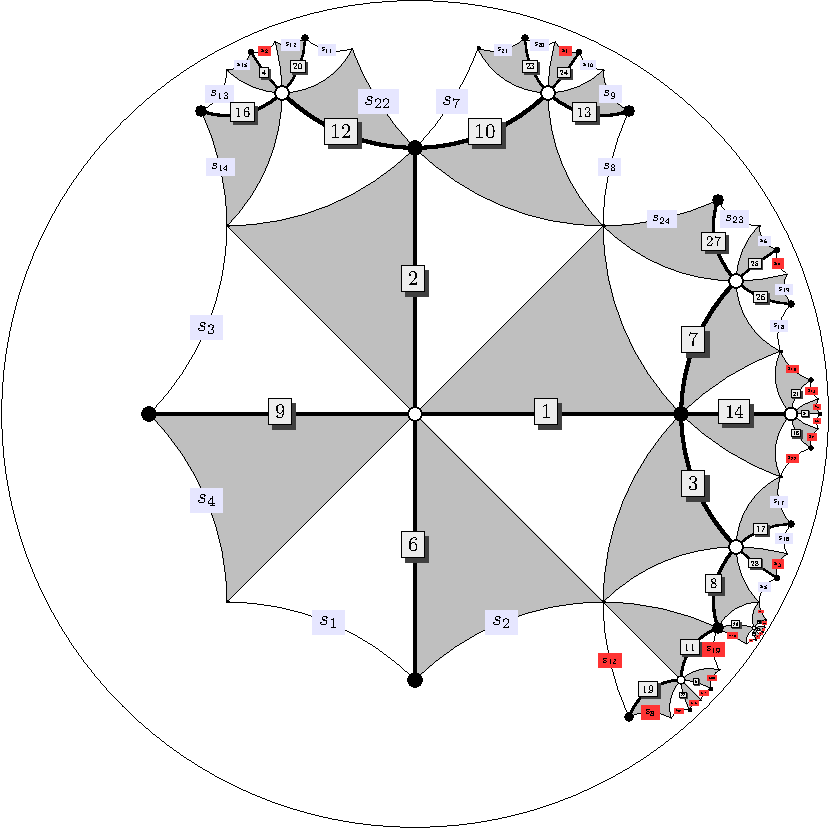
\includegraphics[scale=0.67]{32S2-g5.pdf}
  %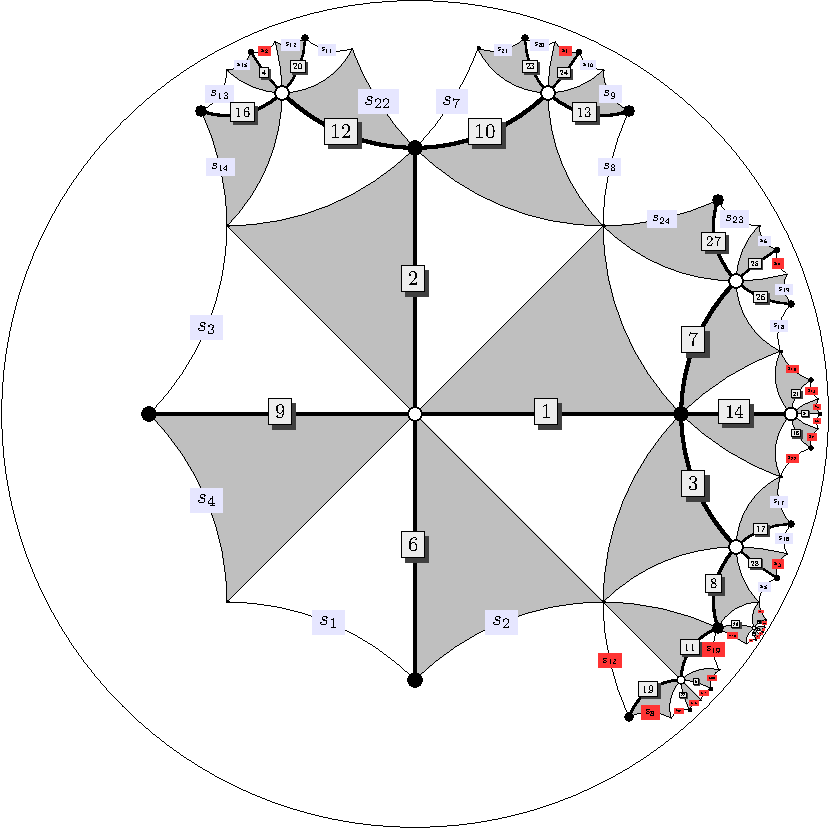
\includegraphics[scale=0.4]{32S2-g5.pdf}
  %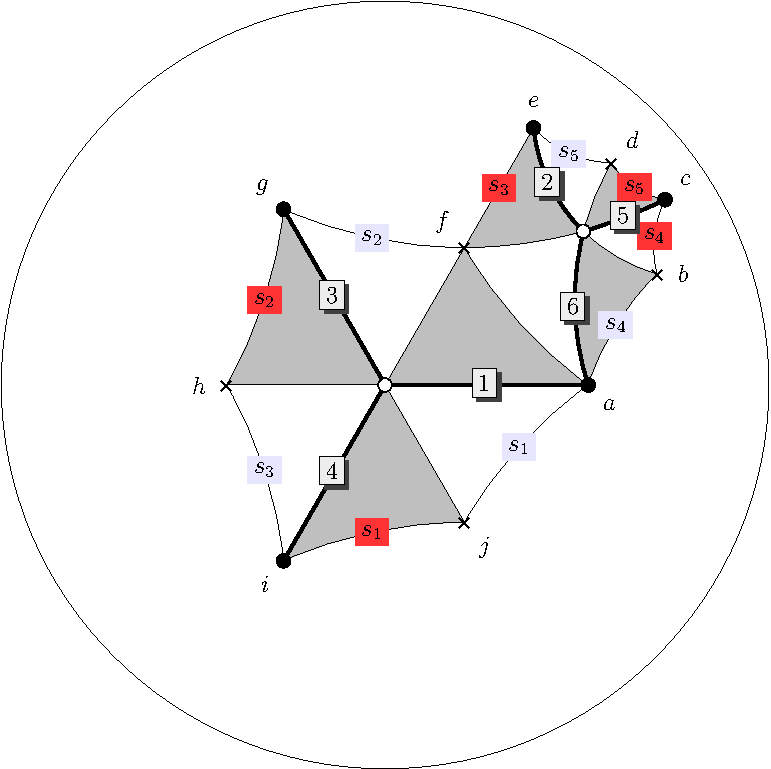
\includegraphics[scale=0.4]{belyi5.pdf}
  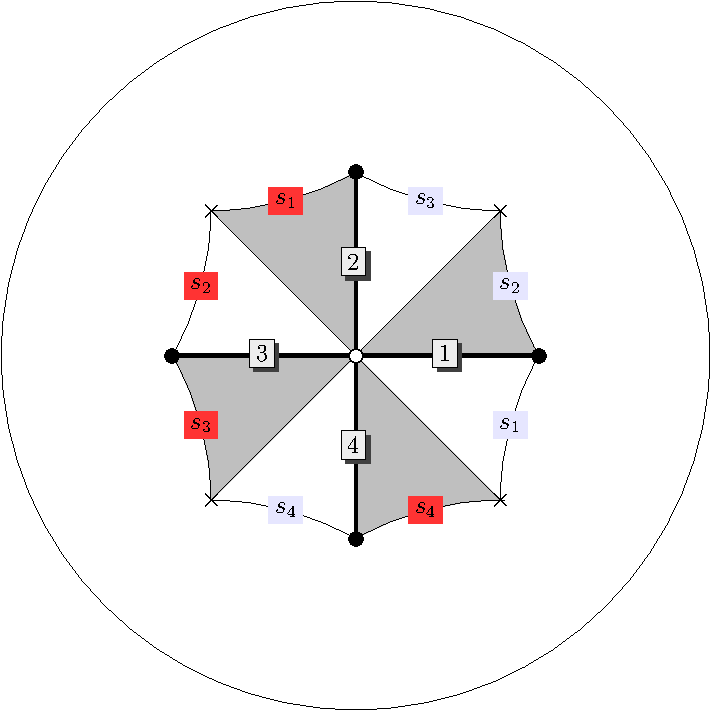
\includegraphics[scale=0.2]{belyi1.pdf}
  \caption{
    A genus 1 dessin d'enfant drawn using \LaTeX and PSTricks.
  }
\end{figure}

\end{document}
